\documentclass[letterpaper, 12pt, oneside]{book}
\usepackage{fullpage}
\usepackage{graphicx}
\usepackage[rightcaption]{sidecap}

\begin{document}

%----------------------------- CHAPTER 1 -------------------------------%
\chapter{}
\section{Background of the Study}
\subsection{Introduction}

	Learning Disabilities are neurologically-based processing problems. Having such condition affects a person’s ability in terms of his learning skills such as reading, writing, processing information, and small instances such as understanding. These disabilities can further interfere with higher level skills such as abstract reasoning, planning, organizing, memory and attention. These abilities not only impacts a person with regards to academic life but also can be a burden to his relationships socially when not given attention early.\newline

Learning Disability is different from learning problem. A person with learning disability has a specific impaired sense which affects a certain aspect on how he learns and processes information. While learning problem isn’t caused by any impairment but rather by the processing capacity of the brain. Persons with disabilities(PWDs) are people with impairment which can be either physical or mental. As of the moment, 10 percent of the world’s population \textit{(which is about 650 million people)} are living with a disability, 30 percent of these belongs to the lower sector of the society or are poor. Two types of learning disabilities in reading involves: the foundational skills required to understand the relationship between letters, sounds, and words; and complex thinking skills such as understanding words, phrases, and larger meanings of passages.\newline

Dyslexia is classified under cognitive disability. This intellectual disability affects problem solving, memory, math comprehension, visual comprehension, reading, visual, verbal, and auditory comprehension. Dyslexia is the most common language-based learning disability. Moreover, Dyslexia is a condition which is inherited and can be found in both male and female regardless of ethnicity. A person suffering from dyslexia may have difficulty in language, reading, spelling and writing. Several related disabilities include Dysgraphia which is a learning disability involving writing capabilities of a person, Dyspraxia, the disability which involves movement and coordination, and Dyscalculia, by it’s name, involves the person’s ability to understand, calculate, and manipulate numeric symbols or numbers.\newline

According to the Department of Education in the Philippines, the number of dyslexics has increased dramatically over the years. This resulted to only few of them being able to reach secondary education or even to graduate in college. As of now, Dyslexia is known to be a condition which does not go away, cannot be outgrown, or cannot be cured by any medical means. Despite all of these, majority of dyslexic patients are exceptionally bright and creative. Some prominent names having Dyslexia includes Regine Velasquez, Tom Cruise, John Lennon, Leonardo da Vinci, Pablo Picasso, Whoopi Goldberg, and even Albert Einstein.\newline
    
\subsection{Background of the Research Area}
	Wordlab is a non-profit organization founded by Ms. Tina de Ocampo who is currently the Undersecretary for Programs of the Department of Education in the country. The institute originally started as a clinic in 1996 practicing the one-on-one school setup to help dyslexic students who are enrolled in traditional schools. The institute is now on their 20th year of operation (2015) and is currently headed by the School Director, Teacher Faye. The institute was first located in Makati but later moved to Mandaluyong, 7th Street, and lastly to its current location in Quezon City.\newline

Wordlab believes that Dyslexia is not a disability but rather is \textit{“just a different way of learning”} for its students. Students who have dyslexia can learn normally since having the condition is not a special case. Based on the observations of the school, Dyslexia is hereditary and is more common on boys (90\% of their students are males). In relation to this, the school concluded that their claim might be possible since the institution currently has a student whose parent was a former student of theirs. To be able to strictly monitor their students, the ratio of teachers to students is 1:2. Currently, the school handles 80 total students (75 boys and 5 girls) with 40 teachers to facilitate them. The teachers must have accomplished the normal requirements required for aspiring educators wherein passing the LET should be one of its priorities. The teachers then undergo a 20-30 day training with Wordlab to be educated and trained in and handling dyslexic students. Wordlab offers primary, middle school and high school levels. They follow the DepEd Curriculum and teaches Araling Panlipunan, Science, Math, English, and Filipino. Since the institution is a private school, Wordlab additionally offers Spelling and Decoding subjects for all levels to focus on addressing Dyslexia. Spelling and Decoding involves phonics, basic symbols, sounds, writing letters on air, writing letters using crayons, letter reversals, and phonograms and spelling exceptions. The level of Spelling and Decoding of each student is based on a student’s level of acquired learning. For example, a student who is currently in its third grade can be in first grade Spelling and Decoding class. Teaching technique is more hands on but still practices the pen-paper method not different from normal schools. Dyslexic students are no different compared to non dyslexic children in terms of technology literacy since they are also able to make use of them normally. Students with processing problems have no external problems so they can go through primary to high school level normally but must build comprehension skills to cope with their difficulty in processing information. For Math subjects, they make use of the Orton-Gillingham Approach, Madrasa Approach for Filipino, and Slingerland Approach for the Reading and Spelling subjects. Students are later tested through written exams. \newline

Students who finish their high school education in Wordlab move on to college level normally. They can go back to Wordlab if they need review or are having trouble adjusting with the traditional school setup. Dyslexia is not a hindrance for patients to become achievers. The institute had students who is now a graduate in College of Music in UP, a theater producer, a licensed engineer, a pilot, and also two previous students who are now teachers in Wordlab.\newline

As for the learning materials, the institute particularly stated that they make use of the Geo Slab and Comic Sans font if technology is needed. The books are created by Wordlab with references from electronic books and school library books.

\subsection{Statement of the Problem}

\subsubsection{Dyslexic students have a hard time distinguishing similar letters from one another.}

	The alphabet consists of 26 letters which are different in pronunciation but may appear similar in presentation. For example, the letter b can be mistaken as p, the letter m can also be mistaken as w and the letters n and u share the same appearance as well. All of these pairs of letters have different orientations in directionality. Students who do not have the learning problem can distinguish these pairs of letters from one another but for the dyslexics, these pairs of letters can bring confusion because of its slight difference in directionality. One letter points upwards while the other letter points downwards. Having a hard time distinguishing similar letters from one another occur due to incorrect visualization of simple symbols such as letters and numbers. The Alphabet is taught in the pre elementary level as one of the most basic lessons essential for further advancement of the students to higher levels. In some cases, dyslexic students also mix up numbers as well. Numbers, such as 7, 1, 8, 0, 6, and 9 also do follow the same slight difference in directionality. Moreover, symptoms for letter reversal result to poor reading and writing skills of the students.

\subsubsection{Dyslexic students cannot easily recognize the different word and letter sounds.}

	Dyslexia is often mistaken as a learning disability in terms of reading and spelling but it is actually a language-based disability wherein the difficulty lies in the phonological sound component of a language. Phonological sound refers to the difficulty in interpreting sounds in words and matching those individual sounds to the letters and combinations of letters in order to read and spell. An individual’s ability to identify and manipulate the individual sounds that  make up words are referred to as phonological skills. Some tasks which use phonological skills are rhyming, having troubles separating individual letter sounds and syllables in a word and identifying how many sounds are there in a word. One of the primary symptoms of dyslexia is that patients with the condition tend to  successfully see or recognize letters but not connect it to the sound they make. For instance, a student might have encountered the word bird but tend to forget or fail to make sense out of it. This results to a repetition of the student to read the passage over and over again. Phonological awareness involves a person’s ability to decompose written or spoken word into individual sounds. For example, a normal child should be able to properly recognize what results if a specific letter is taken away from a word. For example, if we take away \textit{“l”} from the word \textit{“wolf”} and present it to a dyslexic student, he will still recognize it as \textit{“wolf”} since he already encountered the word before rather than be able to distinguish the difference between the two words.

\subsubsection{Dyslexic students cannot easily recognize the different word and letter sounds.}
	
    Dyslexic students often have trouble understanding different words and sentences because they substitute words, omit punctuation marks, add suffixes, prefixes, and pronouns even when it’s unnecessary. Dyslexic students may tend to read single words slowly and inaccurately especially when there are no visual representations. When reading a storybook without illustrations, a dyslexic student may take up too much time understanding words and sentences because of the absence of clues that would give hints to him/her about the story. Also, they often read the wrong words because they assume that a similar word which starts and ends in the same letter are the same. A dyslexic student can also insert or remove letters in a word which he/she have read. For example, a dyslexic reads the word \textit{“form”} as \textit{“from.”} When dyslexic students read, they often forget the punctuation and say a word with the same letters but follows a different sequence. The word “girl” can be read by a dyslexic as \textit{“grill.”} Dyslexic students experience this problem because reading takes up too much time and energy therefore resulting to a low reading comprehension. In view of that, a dyslexic student often substitutes words which look similarly hence changing the meaning of a sentence that he/she is reading. 
    
\subsubsection{Dyslexic students have problems recognizing phonograms and spelling exceptions.}

	The English language is derived from many languages such as Greek, Latin and French hence many English sounds can be spelled in many different ways. Learning to spell English words is difficult because each sound can be represented in various ways. However, spelling in English can be predicted  because of the different spelling rules and patterns. With that being said, the ability to spell is hard to learn because of an individual must have good knowledge in roots, suffixes, prefixes and morphological structures. Before trying to spell, an individual must be able to know how the word should be deconstructed, it can either be at the syllable level, phonemic level or the orthographic level. When an individual spells, a word is manipulated, broken down into its individual sounds and then transform those individual sounds into letters or letters representing each sound. Dyslexic students have difficulties with syllables and identifying word and letter sounds therefore having problems with spelling and identifying spelling exceptions as well.\newline

	Phonograms refers to letter combinations which makes up a sound. This may not only be limited to two letters and can sometimes be in groups of threes. For example, the word pick comprises of p-i-c- and k. The letters c and k forms a single sound which can be related to the sound of c or k. \textit{“High”} is composed of h-i-g- and h but -igh share the similar sound with the long i. Another example is the word “edge”. the \textit{“dge”} basically sounds as the letter \textit{“j”} so if spelling isn’t taken into consideration, it will sound same to a text written as \textit{“ej”}. These letter and spelling exceptions may bring confusion to dyslexic students since they basically sound the same. Even though these words or letters share the same sound, that doesn’t mean it should be allowed to be spelled in any way a person interprets it. Flew and Flu share similar pronunciation but has different meanings. Dyslexic students are challenged in learning these basic grammar rules since they have poor phonological skills. %revise problems

%----------------------------- CHAPTER 2 -------------------------------%
\chapter{}
\section{Review of Related Literature}
\subsection{Related Concepts}
\subsubsection{Dyslexia}
Dyslexia is a type of learning disability which causes difficulty in reading and processing words. People with dyslexia experience trouble learning to read even though they are smart enough to do so. Dyslexia is not considered to be a disease, thus, is considered as a condition and in most cases, hereditary. Most people think of Dyslexia as a condition in which patients sees words backwards and reverses or interchanges similar looking letters. Reversal only occurs in the developmental stage of a patient but can later be overcome and still be dyslexic. Moreover, dyslexia affects phonological awareness, word processing, auditory short term loss and rapid naming. 

\subsubsection{Phonological and Phonemic Awareness}
Phonological awareness consists of awareness in sounds in a specific language, awareness to rhymes, and awareness that sentences can be broken down into words, and later into syllables. It also refers to the ability to manipulate sounds and being able to understand the connection between written and spoken word. A person’s phonological awareness initially develops in the preschool stage and is later improved through training and exposure to speech, vocabulary, sounds, and such. 

\subsubsection{Reversal}
Reversal is often experienced by dyslexic patients. To a person with dyslexia, words can appear jumbled when read. In some cases, uppercase letters are viewed same as lowercase letters. For instance, the letter \textit{“i”} for a dyslexic patient can also be seen as \textit{“j”}, letters \textit{“b”} and \textit{“d” }appear similar to them, and symbols with noticeable similarities such as letters \textit{“n”} and \textit{“h”} are perceived similarly. 

\subsubsection{Developmental Reading Disorder}
Developmental Reading Disorder is another term for Dyslexia or \textit{“alexia”}. It is the most commonly diagnosed learning disability, it occurs when your brain has a hard time processing language. Misreading letters in a word or having the difficulties in reading unfamiliar words are its most common symptoms. This kind of disorder is often identified when a child reaches first grade. Children who is diagnosed with reading disabilities are often left behind by their peers during activities which require reading and spelling. Treating children with developmental reading disorder varies depending on the quality of the reading program, severity of the disorder and the motivation and intelligence of the child. 

\subsubsection{Auditory Processing Disorder}
Auditory Processing Disorder is also known as Central Auditory Processing Disorder. Children with Auditory Processing Disorder have difficulty processing the information they hear because their ears and brains have bad coordination. Children diagnosed with this disorder cannot fully recognize the difference between sounds in words regardless of its volume. Processing auditory information is hard for children who are diagnosed with this disorder. Auditory Processing Disorder is part of the identification process of diagnosing children with dyslexia. Children who are diagnosed with dyslexia should take a series of tests first in order to be fully recognize if it is dyslexia or auditory processing disorder. 

\subsubsection{Phonological Processing}
Phonological Processing is the understanding of sounds used in language which ranges from words to syllables and to every available sound within a syllable. It is an auditory processing skill which should be taught before letters are introduced. Implementing Phonological processing creates the link between the letters and its individual sounds which can be used for both reading  and spelling. 

\subsubsection{Orthographic Awareness}
Orthographic Awareness is being sensitive towards the structure of the writing system such as spelling patterns, orthographic rules, inflectional and derivational morphology and etymology. In relation to that, orthographic awareness is having the difficulty visualizing letters therefore having problems in reading and spelling. It also affects the ability of recognizing root words. If a letter’s orientation is not instilled in an individual’s visual memory, this individual tends to reverse letters and will have the difficulty in recognizing that the letters are wrong.


\subsubsection{Assistive Technology}

Assistive technology \textit{(often abbreviated as AT)} is any item, piece of equipment, software or product system that is used to increase, maintain, or improve the functional capabilities of individuals with disabilities. Assistive technology offers a way for dyslexics to save time and overcome some of the issues they may encounter because of their dyslexia, such as slow note taking or unreadable handwriting, and allows them to use their time for all the things in which they are gifted. For dyslexic students, technology opens doors and allows them to demonstrate their knowledge in ways that were unimaginable in the past. Two technologies that facilitate this process are the \textit{Livescribe smartpen} and \textit{Dragon Naturally Speaking}. Each aide is designed to make the learning process easier and each offers support to the dyslexic student in different ways.

\subsubsection{Orton-Gillingham Approach}
It is diagnostic and prescriptive. Each lesson is planned for a particular student or small group of students. It is not a \textit{“packaged”} curriculum in which “one size fits all.” The teacher must be adaptable and flexible, understanding the learner’s needs and using appropriate teaching strategies. Orton-Gillingham is also direct and explicit, and students are not expected to know anything that has not already been taught and practiced. It is language based. Teachers are trained in the structure of the English language. They teach the language as it is to the students where they are in their understanding of the language. Many programs say that they employ multisensory methods but to be truly multisensory, Teachers must make sure that auditory, visual and kinesthetic elements are utilized together to reinforce each element for optimal learning. What makes Orton-Gillingham unique in this respect is that spelling is taught simultaneously with reading. It is critical that reading and spelling go hand in hand.

\subsubsection{Slingerland Approach}
The Slingerland Approach is a structured, simultaneous multisensory, alphabetic-phonic methodology that explicitly teaches the concepts of written language including the correct stroke order and formation of handwriting for both manuscript and cursive letters, sound/symbol relationships, strategies for spelling and decoding, spelling generalizations, studying red flag/non-phonetic words, meanings to suffixes and prefixes, phrase/sentence writing, editing strategies, reading in meaningful phrases, and reading for meaning. Slingerland uses the three modalities of auditory, visual, and kinesthetic-motor to ingrain individual concepts into long-term memory.

\subsubsection{Madrasa Approach}
Madrasa Approach is a learning technique which originated in the Muslim community. This technique uses rote memorization and chanting words and sentences repeatedly in order for a student to learn about the basics of the Islam and Arabic language. Today, geography, history, science and math can also  be taught if the teacher has sufficient knowledge about these sciences. Moreover, the said approach is also used worldwide not only in traditional school science subjects, languages and also, to instill values and nationalistic views.

\subsubsection{Dyslexie}
Dyslexie is a font developed by Christian Boer. Originally, the font was developed as his final thesis project. Boer’s goal was to make digital reading of text easier especially for people having Dyslexia. What makes Dyslexie effective is that the similar looking alphabets are tweaked in a way that it will be distinctly recognizable. Instances such as the letter j is slightly slanted so that dyslexics won’t mistaken it as the letter i, the letter l has a small hook like tail, and such. The font is now widely used today and is offered free for all in their website.

\subsubsection{Davis Approach}
The Davis approach cures the problem of all learning difficulties. The approach aims to cure disorientation which can be controlled at a student’s own will. The said approach uses the multisensory design as well. Dyslexics think using pictures hence always looking at the bigger picture, missing out on all of  the important small details which often results to wrong generalizations. Symbols such as letters and numbers therefore becomes a hard object to understand for a dyslexic because of disorientation. The Davis approach therefore cures disorientation, does not use rote memorization as a means of learning but using a mental picture to teach a symbol. 

\subsubsection{Phono-Graphix Approach}
The Phono-Graphix Approach is an instructional method which focuses on phonemic awareness. It is an approach that follows a structured, systematic and multisensory design in order to teach words. The said approach teaches from sound to symbol. For example, the sound /ch/ will be represented as ch or tch. The instructional method emphasizes that letters are visual representations or “pictures” of a sound in words. It uses Segmenting, Blending and Phoneme Manipulation. Pictures are for a specific sound are taught starting from the simplest to the least common. 

\subsubsection{Elaboration Theory}
Elaboration theory is an instructional design theory which groups information that should be learned from simple to complex for learning to be more effective. The increasing order of complexity produces a more optimized way of learning, helps in such a way that it attains learning goals faster. In a discussion, simplest task is given to the student, then the level of difficulty of the task increases subsequently until the task is completely accomplished. These tasks can be accomplished through the use of motivators and analogies, and all acquired learning including from the previous tasks must be remembered and concluded through the use of summaries and syntheses. Applying this theory would result to a more stable cognitive structures hence better retention, a continuously motivated learner and proper learner control. The theory therefore values how instructions are presented. 

\subsubsection{Multi-sensory teaching}
Multi-sensory teaching allows learning to occur by engaging the students to use all of their senses to gather information about a specific task, create a link between previous knowledge and new knowledge to be acquired, perceive the logic which can be used to solve problems, learn and store information. Techniques which fall under the multi-sensory teaching allows a student with a learning disability to use his/her own strengths in learning. Visual methods such as text, pictures, posters and computers are used in this teaching style. Finger spelling, use of different colors for highlighting words and charts also fall under the visual category. For auditory, clay modelling, building puzzles and finger painting are activities which stimulate multi-sensory teaching as well. Lastly, activities which require motor skills fall under kinesthetics. 

\subsection{Related Systems}
\subsubsection{Dragon Naturally Speaking}
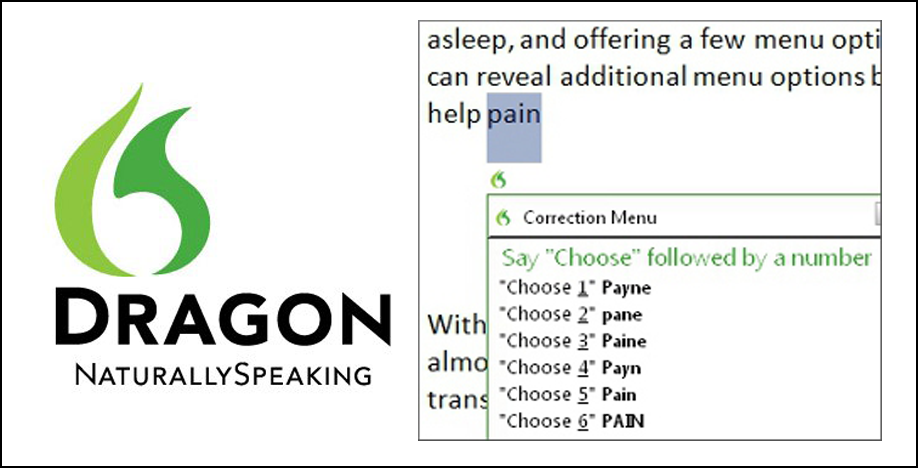
\includegraphics[width=\textwidth]{dragon}
\newline
Dragon Naturally Speaking is a technological aid computer software addressed for people having word-retrieval problems, grapho-motor or handwriting weaknesses, and difficulties in transferring ideas to paper. Dragon is basically a speech recognition program which transforms dictated speech to text in the computer. The software initially requires the users to create a profile and follow a series of steps in order for Dragon to analyze the user’s accuracy. It does not only gauge the user but also adjusts for them since there are ranged levels of words to be read so that the program can level the user more accurately.

\subsubsection{Clicker 6}
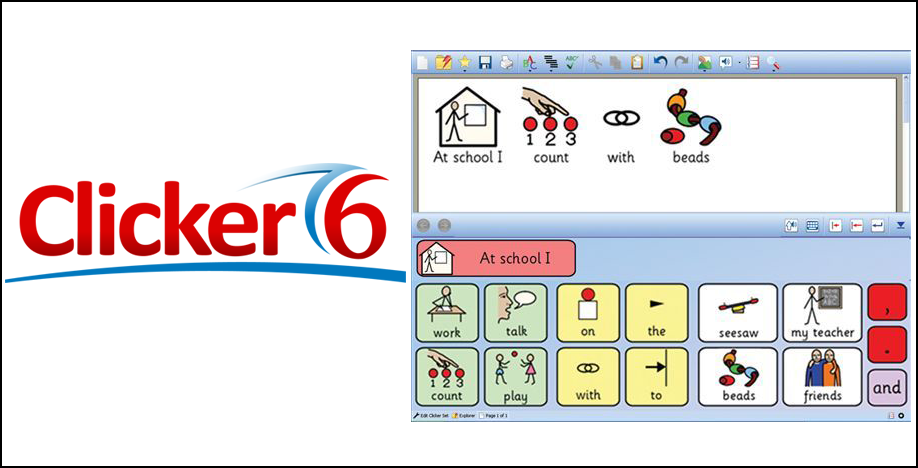
\includegraphics[width=\textwidth]{clicker6}
\newline
Clicker 6 is a software developed by Crick, a company specialized in developing reading and writing software for children. Clicker is a word processor which enabled children to construct and write sentences through clicking rather than typing. Clicker features intelligent word prediction to solve users with spelling difficulty. Clicker also has a speech feedback wherein constructed sentences are read aloud to enable the users to detect corrections. 

\subsubsection{iReadWrite}
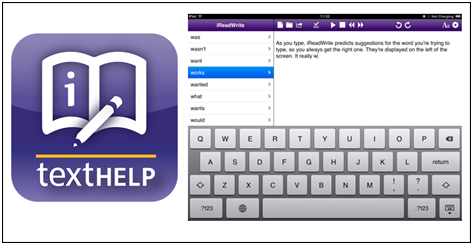
\includegraphics[width=\textwidth]{ireadwrite}
\newline
iReadWrite is an iPad application by Texthelp addressed to users with dyslexia and dysgraphia. iReadWrite shares similar features with Clicker 6 such as word prediction and click and drag features in order to construct sentences. Additionally, iReadWrite has a feature to highlight grammatical errors and words that look and sound the same. These highlighted words are clickable and prompts the user into the application’s built-in dictionary for checking. Lastly, the application can import documents and convert it into editable format for the user.

\subsubsection{Click n' Read}
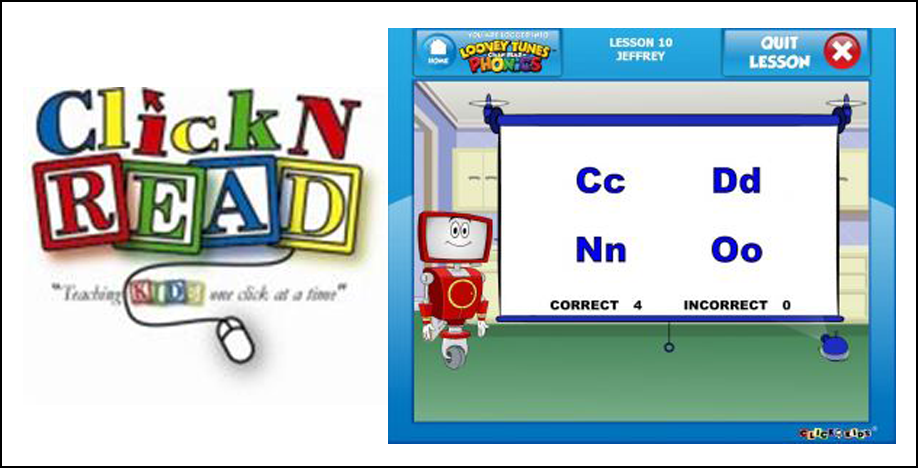
\includegraphics[width=\textwidth]{clicknread}
\newline
Click n Read is a computer based program that is designed to teach phonics curriculum for  in kindergarten through third grade. It was developed based on educational research. Interactive animated cartoons are being used to teach each lesson. The use of graphics will motivate the program’s users which are children ages 7-9 yrs old. Click n Read is guided by a character to build a very user-friendly interaction between the program and the user. It comprises of 100 lessons which can all be learned by the user without supervision. 

\subsubsection{Read, Type \& Spell Well}
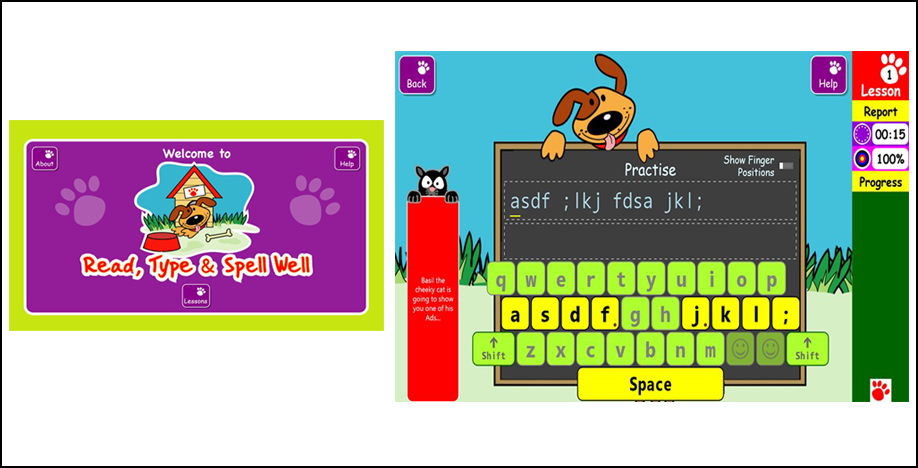
\includegraphics[width=\textwidth]{rwsw}
\newline
Read, Type \& Spell Well is a software designed for children which improves the user’s accuracy in typing. Several lessons include typing letters, numbers, and even symbols depending on what is displayed on the screen. The user is gauged by time and the number of characters they got right. Instructions are voiced to give ease to the dyslexic users and lessen reading. Word and sentence building is also taught through the program. For example, the software asks the user to type “ask the lad”, before requiring the phrase itself, the software requests the user to repeatedly type “ask” first and the word is later voiced which also improves vocabulary and auditory awareness.

\subsubsection{Nessy Reading Spelling}
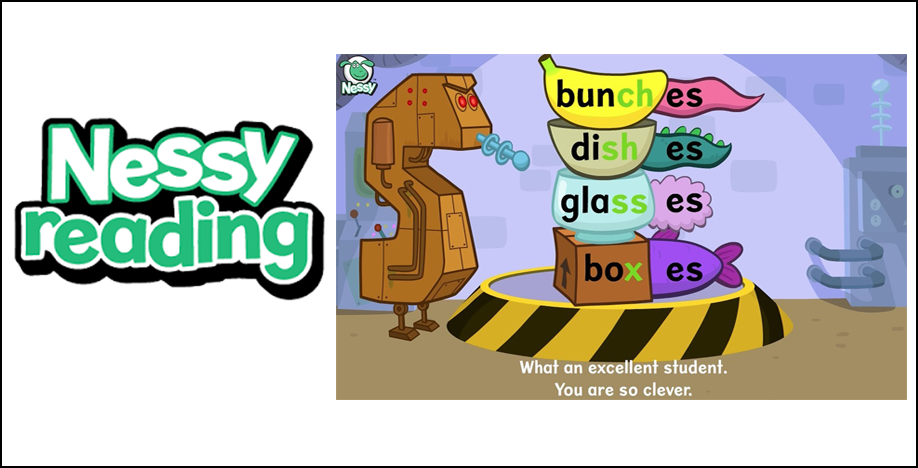
\includegraphics[width=\textwidth]{nesssy}
\newline
Nessy Reading Spelling is a subscription-based application that teaches the basics of reading comprehensively. Through the use of animated reading and spelling strategies, the students are inherently being taught on prefixes and suffixes, phonemes, mnemonics and memory strategies.

\subsubsection{Read \& Write Toolbar}
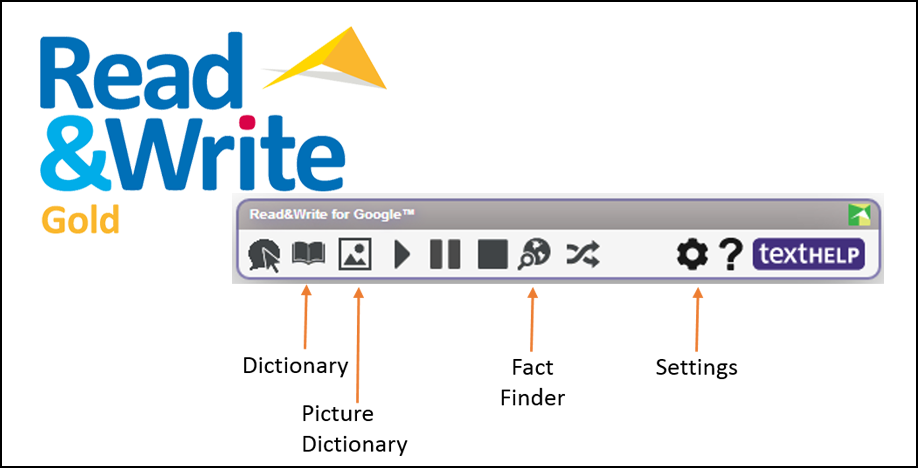
\includegraphics[width=\textwidth]{toolbar}
\newline
Read \& Write Toolbar is a desktop application that provides dyslexics literacy support through the use of easy-to-use toolbar. This application is a reading aid with features \textit{hover speech} that acts as a  for readers who are having a difficulty reading blocks of text in %add details STILL INCOMPLETE

\subsubsection{BigKeys Keyboard}
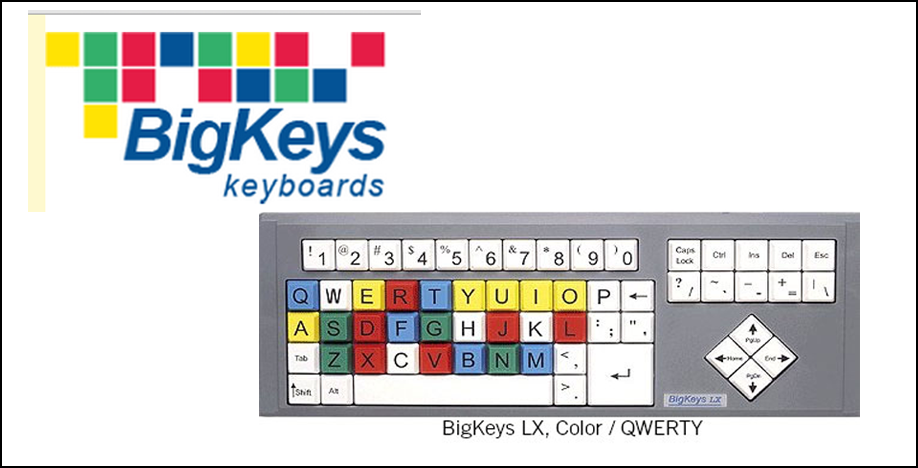
\includegraphics[width=\textwidth]{bkeybord}
\newline
BigKeys keyboards are simplified computer keyboards. They are the same size as a standard keyboard, have fewer keys and extra large sized keytops. The large keys and simple layout of the BigKeys Plus keyboard help users explore letters and words without confusion. The simplified keyset avoids ambiguity and deflects interference with the computer. Not only is this ideal for early learners of all ages but can be of great assistance with dyslexia and related learning difficulties.

\subsubsection{Reading Enhancement Aid for Dyslexics}
Reading Enhancement Aid for Dyslexics is an undergraduate thesis developed by students from the College of Computer Studies. The aforementioned thesis is a desktop-based courseware that teaches digraph rules to elementary level students.

\subsection{Concept Map based on Review of Related Literature}






















\end{document}